\section{Vision Transformer}

Originalna Transformer arhitektura, koju su uveli Vaswani i saradnici \cite{vaswani2017attention}, inicijalno je razvijena za obradu prirodnog jezika. Prepoznajući njen potencijal, Dosovitskiy i saradnici \cite{dosovitskiy2021vit} adaptirali su ovaj koncept za računarsku viziju uvođenjem \textit{Vision Transformer} (ViT) modela, gde se slika posmatra kao sekvenca tokena. U nastavku su detaljno opisane ključne komponente ove arhitekture.

\subsection{Patch Embedding}
\label{sec:patch_emb}
Pošto je Transformer arhitektura primarno dizajnirana za rad sa sekvencama, prvi korak pri njenoj primeni na slike jeste transformacija dvodimenzionalnih vizuelnih podataka u jednodimenzionalnu sekvencu vektora. ViT to postiže podelom ulazne slike dimenzija $H \times W \times C$ na $N$ nepreklapajućih pečeva (\textit{patches}) fiksne veličine $P \times P$, gde je broj dobijenih pečeva definisan kao:

\begin{equation}
    N = \frac{H \cdot W}{P^2}
\end{equation}

Svaki peč se potom vektorizuje u niz dimenzije $P^2 \cdot C$ i linearno projektuje u prostor dimenzije $D$, koja predstavlja dimenziju modela (\textit{embedding dimension}). Ova linearna projekcija se u praksi efikasno realizuje pomoću konvolucionog sloja sa dimenzijom filtera i preskokom (\textit{stride}) jednakim $P$. Ovaj proces je matematički ekvivalentan operaciji vektorizacije i množenja matricom težina:

\begin{equation}
    \mathbf{z}_i = \mathbf{W}_E \cdot \text{flatten}(\mathbf{x}_i) + \mathbf{b}_E, 
    \quad i = 1, \ldots, N
\end{equation}
gde je $\mathbf{W}_E \in \mathbb{R}^{D \times (P^2 \cdot C)}$ matrica projekcije, a $\mathbf{x}_i$ označava $i$-ti peč ulazne slike.

U slučaju standardnog ViT-Base modela koji se koristi u ovom radu, ulazna slika dimenzija $224 \times 224$ piksela deli se na pečeve veličine $16 \times 16$. Primenom gornje formule dobija se sekvenca od:

\begin{equation*}
    N = \frac{224 \times 224}{16^2} = 196
\end{equation*}
vektora, odnosno vizuelnih tokena. Celokupna struktura modela i tok podataka detaljnije su prikazani na slici \ref{fig:vit_architecture}.

\begin{figure}[htbp]
    \centering
    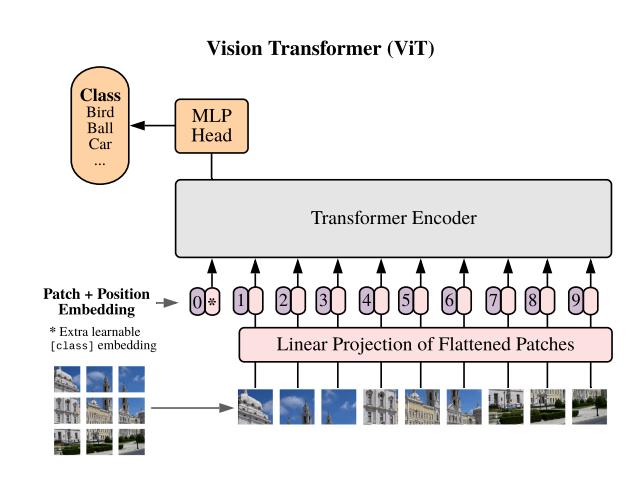
\includegraphics[width=0.7\textwidth]{figures/ViT/vit_architecture.png}
    \caption{Arhitektura Vision Transformer modela. Preuzeto iz \cite{dosovitskiy2021vit}.}
    \label{fig:vit_architecture}
\end{figure}

\subsection{CLS Token}

Pre prosleđivanja sekvence pečeva kroz Transformer enkoder, sekvenci se dodaje poseban naučeni parametar — \textit{CLS} token (\textit{classification token}), čiji je koncept preuzet iz BERT arhitekture \cite{devlin2019bert}. Spajanjem vektora \textit{CLS} tokena $\mathbf{z}_{cls} \in \mathbb{R}^D$ sa linearno projektovanim vektorima pečeva formira se početna sekvenca koja se prosleđuje modelu.

Za razliku od ostalih tokena koji reprezentuju specifične lokalne delove slike, \textit{CLS} token nema prostorno značenje niti je vezan za bilo koji konkretan region. Njegova uloga je da kroz slojeve enkodera, putem mehanizma pažnje, agregira relevantne informacije iz svih ostalih vizuelnih tokena duž cele sekvence. Na izlazu iz enkodera, stanje ovog specifičnog tokena služi kao kompaktna, globalna reprezentacija cele slike.

\subsection{Positional Embedding}
\label{sec:posemb}
Mehanizam pažnje po svojoj prirodi ne uzima u obzir redosled elemenata u sekvenci, već svaki token interaguje sa svim ostalima potpuno ravnopravno. Kako bi model zadržao informaciju o prostornom rasporedu pečeva na originalnoj slici, svakom vizuelnom tokenu se dodaje odgovarajući pozicioni vektor:

\begin{equation}
    \mathbf{z}_i \leftarrow \mathbf{z}_i + \mathbf{e}_i^{pos}, \quad i = 0, 1, \ldots, N
\end{equation}
gde $\mathbf{e}_i^{pos} \in \mathbb{R}^D$ predstavlja naučeni pozicioni vektor, koji se pridružuje svakom tokenu, uključujući i specijalni \textit{CLS} token. 

Za razliku od originalnog Transformer modela koji se oslanja na fiksne sinusoidalne funkcije, ViT koristi naučene jednodimenzionalne (1D) pozicione vektore. To znači da svaki token dobija jedinstven vektor položaja, bez potrebe za eksplicitnim kodiranjem dvodimenzionalne geometrije same slike.


\subsection{Mehanizam Pažnje}
\label{sec:attention}
Centralna komponenta ViT arhitekture je mehanizam višestruke pažnje (\textit{Multi-Head Self-Attention} - MHSA). U ovom mehanizmu, svaki token iz ulazne sekvence se projektuje u tri različita vektora: upit (\textit{query}, $\mathbf{Q}$), ključ (\textit{key}, $\mathbf{K}$) i vrednost (\textit{value}, $\mathbf{V}$):

\begin{equation}
    \mathbf{Q} = \mathbf{Z}\mathbf{W}^Q, \quad 
    \mathbf{K} = \mathbf{Z}\mathbf{W}^K, \quad 
    \mathbf{V} = \mathbf{Z}\mathbf{W}^V
\end{equation}
gde su $\mathbf{W}^Q, \mathbf{W}^K, \mathbf{W}^V \in \mathbb{R}^{D \times d_k}$ naučene matrice projekcije. Ovde $h$ označava ukupan broj komponenti pažnje, dok je $d_k = D / h$ dimenzija prostora u koji projektuje svaka pojedinačna komponenta.

Unutar svake komponente, funkcija pažnje se računa preko skaliranog skalarnog proizvoda (\textit{Scaled Dot-Product Attention}):
\begin{equation}
    \text{Attention}(\mathbf{Q}, \mathbf{K}, \mathbf{V}) = 
    \text{softmax}\left(\frac{\mathbf{Q}\mathbf{K}^T}{\sqrt{d_k}}\right)\mathbf{V}
\end{equation}
\begin{figure}[htbp]
    \centering
    \begin{minipage}[b]{0.47\textwidth}
        \centering
        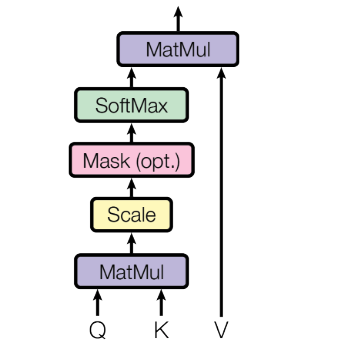
\includegraphics[width=\textwidth]{figures/ViT/attention_mechanism.png}
        \caption{Mehanizam skalirane pažnje (\textit{Scaled Dot-Product Attention}). Preuzeto iz \cite{vaswani2017attention}.}
        \label{fig:attention}
    \end{minipage}
    \hfill 
    \begin{minipage}[b]{0.47\textwidth}
        \centering
        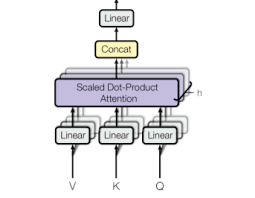
\includegraphics[width=\textwidth]{figures/ViT/multihead_attention.png}
        \caption{Višestruka pažnja (\textit{Multi-Head Attention}). Preuzeto iz \cite{vaswani2017attention}.}
        \label{fig:multihead}
    \end{minipage}
\end{figure}

Matrica $\mathbf{A} = \text{softmax}\left(\frac{\mathbf{Q}\mathbf{K}^T}{\sqrt{d_k}}\right) \in \mathbb{R}^{(N+1) \times (N+1)}$ predstavlja takozvanu matricu pažnje (\textit{attention matrix}). Element $a_{ij}$ ove matrice kvantifikuje meru u kojoj token $i$ uzima u obzir informacije iz tokena $j$ prilikom formiranja svoje izlazne reprezentacije. Budući da se softmax funkcija primenjuje nezavisno po redovima, zbir elemenata u svakom redu matrice pažnje jednak je jedinici:

\begin{equation}
    \sum_{j=0}^{N} a_{ij} = 1, \quad \forall i
\end{equation}

Ove vrednosti se mogu interpretirati kao raspodela verovatnoće, odnosno udeo „pažnje” koji token $i$ usmerava ka svakom od preostalih tokena u sekvenci. Upravo zbog ove intuitivne interpretacije, težine unutar matrice pažnje predstavljaju prirodan izbor za vizuelizaciju i analizu odluka modela, pružajući direktan uvid u to na koje se regione slike model najviše oslanja.

Deljenje sa $\sqrt{d_k}$ vrši se radi stabilnosti treninga — bez skaliranja, 
skalarni proizvodi mogu postati veliki za visoke dimenzije, što dovodi do zasićenja 
softmax funkcije i nestajanja gradijenata.

\subsubsection{Višestruka Pažnja}

Umesto jedne matrice pažnje, ViT koristi $h$ paralelnih komponenti pažnje, od kojih svaka uči specifične projekcije i time omogućava modelovanje različitih vrsta zavisnosti između tokena \cite{voita2019analyzing}:

\begin{equation}
    \text{MHSA}(\mathbf{Z}) = \text{concat}(\text{head}_1, \ldots, \text{head}_h)\mathbf{W}^O
\end{equation}
gde $\mathbf{W}^O \in \mathbb{R}^{D \times D}$ predstavlja matricu izlazne projekcije. Istraživanja su pokazala da se pojedinačne komponente pažnje specijalizuju za različite aspekte unutar podataka — dok se neke fokusiraju na lokalne zavisnosti i fine detalje, druge prate globalne strukture i širi kontekst \cite{voita2019analyzing}.

\subsection{Mreža unapred po pozicijama}

Nakon bloka sa višestrukom pažnjom, reprezentacija svakog tokena se nezavisno procesira kroz mrežu unapred (engl. \textit{Feed-Forward Network}, FFN), koja se primenjuje izolovano na svaki pojedinačni token:

\begin{equation}
    \text{FFN}(\mathbf{z}) = \mathbf{W}_2 \cdot \text{GELU}(\mathbf{W}_1 \mathbf{z} + \mathbf{b}_1) + \mathbf{b}_2
\end{equation}
gde su $\mathbf{W}_1 \in \mathbb{R}^{4D \times D}$ i $\mathbf{W}_2 \in \mathbb{R}^{D \times 4D}$ 
naučene matrice, dok su $\mathbf{b}_1$ i $\mathbf{b}_2$ odgovarajući vektori pomeraja. Ključna osobina FFN sloja je da tokeni međusobno ne komuniciraju — 
svaki token se transformiše isključivo na osnovu sopstvene reprezentacije. Sva 
interakcija između tokena odvija se isključivo kroz mehanizam pažnje.

\subsection{Transformer enkoder i klasifikacija}

Kompletni Transformer enkoder sastoji se od $L$ identičnih blokova. Svaki blok sadrži sloj sa višestrukom pažnjom i sloj mreže unapred po pozicijama (FFN), pri čemu su oba sloja praćena normalizacijom po slojevima (\textit{Layer Normalization}, LN) i rezidualnim vezama:

\begin{equation}
    \mathbf{Z}'_l = \text{MHSA}(\text{LN}(\mathbf{Z}_{l-1})) + \mathbf{Z}_{l-1}
\end{equation}

\begin{equation}
    \mathbf{Z}_l = \text{FFN}(\text{LN}(\mathbf{Z}'_l)) + \mathbf{Z}'_l
\end{equation}

Rezidualne veze imaju fundamentalnu ulogu u stabilizaciji procesa treniranja dubokih 
mreža jer omogućavaju direktan protok gradijenata kroz arhitekturu, čime se ublažava 
problem njihovog nestajanja \cite{he2016resnet}. Pored toga, iz perspektive 
interpretabilnosti i analize toka informacija, ove veze obezbeđuju očuvanje identiteta 
i bazičnih odlika tokena kroz slojeve, sprečavajući da se njihove jedinstvene informacije 
potpuno izgube ili previše uniformno izmešaju tokom operacija pažnje i nelinearnih 
transformacija.

Nakon prolaska kroz svih $L$ blokova, izlazna reprezentacija klasifikacionog (\textit{CLS}) tokena, označena kao $\mathbf{z}^L_{cls}$, prosleđuje se kroz linearni klasifikacioni sloj:

\begin{equation}
    \hat{y} = \text{softmax}(\mathbf{W}_{head} \cdot \mathbf{z}^L_{cls} + \mathbf{b}_{head})
\end{equation}

Konačna odluka modela donosi se isključivo na osnovu reprezentacije \textit{CLS} tokena. Ovaj token kroz slojeve akumulira globalne informacije o celokupnom sadržaju slike, ostvarujući interakciju sa svim preostalim tokenima delova slike putem mehanizma pažnje. U ovom radu korišćena je ViT-Base arhitektura modela, koju karakteriše $L=12$ blokova enkodera, $h=12$ komponenti pažnje i skrivena dimenzija modela $D=768$.

\subsection{Maskiranje tokena}
\label{sec:masking}
Jedna od ključnih osobina Transformer arhitekture jeste način na koji 
tokeni međusobno komuniciraju. Kao što je opisano u sekciji \ref{sec:attention}, 
jedini mehanizam interakcije između tokena je mehanizam pažnje.

Ova osobina ima važnu posledicu: ukoliko se uticaj određenog tokena na 
ostale tokene postavi na nulu u mehanizmu pažnje, taj token efektivno prestaje 
da postoji za ostatak mreže. Formalno, maskiranje tokena $j$ postiže se 
postavljanjem odgovarajuće kolone matrice sirovih skorova pažnje na $-\infty$ 
pre softmax normalizacije:

\begin{equation}
    \tilde{S}_{ij} = 
    \begin{cases}
        S_{ij} & \text{ako token } j \text{ nije maskiran} \\
        -\infty & \text{ako je token } j \text{ maskiran}
    \end{cases}
\end{equation}
gde je $\mathbf{S} = \mathbf{Q}\mathbf{K}^T / \sqrt{d_k}$ matrica sirovih 
skorova pažnje, a $\mathbf{A} = \text{softmax}(\tilde{\mathbf{S}})$. Nakon 
softmax normalizacije, maskirani tokeni dobijaju težinu nula u svim redovima 
matrice pažnje, što znači da nijedan drugi token ne prima informacije od njih. 
Na ovaj način se postiže čisto izolovanje pojedinih pečeva slike bez potrebe 
za popunjavanjem ili bilo kakvom modifikacijom ulazne slike.